%UV emission lines generally require high excitation and ionization conditions, and the strength of emission correlates with gas excitation, as probed by optical \oiii transitions \citep{Berg+2016}.

%Observations of low redshift galaxies have established a relationship between galaxy stellar mass, metallicity, and SFR, controversially ref called the "fundamental relation" (Ellison+2008, Mannucci+2010, LaraLopez+2010). At redshifts between 1 and 3, the nature of the FMR is uncertain. Some studies find a constant FMR at all metallicities (Wuyts et al. 2012,Henry et al. 2013; Hunt et al. 2016) while others find a FMR that evolves with redshift (Zahid et al. 2014; Grasshorn Gebhardt et al. 2016; Kashino et al. 2017).
%Our understanding of gas properties in the earliest galaxies remains primitive. This is exacerbated by our lack of tools; at redshifts above $z{\sim}5$, the well-established optical diagnostics are observationally inaccessible with ground-based optical and IR facilities. To probe the physical conditions of the gas in these early galaxies, we must instead rely on emission line diagnostics that originate in the ultra-violet (UV) part of the spectrum.

% AYAN'S PAPER LINES

The continuum is fit using an automatic routine that first masks the spectrum at the positions of expected spectral features (which includes emission and absorption lines in addition to known intervening absorption systems), and then applies boxcar smoothing. The resulting continuum is nearly identical to the hand-fit spline process described in \citet{Rigby+2018a}.

Emission lines are fit to the continuum-normalized spectrum. Gaussian profiles are fit to each emission line of interest using {\tt scipy.optimize.curve\_fit}; neighboring emission lines (lines within $\pm 5$ spectral elements) are fit simultaneously. Initial guesses for line centers are calculated by redshifting the emission line vacuum wavelength to the nebular redshift, calculated in \citet{Rigby+2018a} using the \ciii$\lambda$1906,1909 lines. Limits on the center of the Gaussian profile are set to $\lambda \times (1 \pm 3\sigma$, where $\sigma$ is the $1\sigma$ uncertainty on the nebular redshift. The width of the Gaussian profile has lower and upper limits of d$\lambda$ (one spectral resolution element) and 300\kms, respectively.

Some emission lines are affected by intervening absorption lines. The intervening absorption features are fit simultaneously with the emission lines to properly account for the absorbed emission line flux.

For each emission line flux, $f_{\mathrm{line}}$, we determine the significance of the line following the methodology presented in \citet{Schnieider+1993}. We first compute the rolling average of the error-weighted flux as a function of wavelength, $f_{\mathrm{Schnieder}}$. We then compute the significance of a given emission line, $f_{\sigma}$, as the ratio between the measured emission line flux, $f_{\mathrm{line}}$, and $f_{\mathrm{Schnieder}}$ computed at line center. If $f_{\sigma}>3$ and $\SN > 1$, the emission line is considered ``detected''. Emission lines not meeting this criteria are considered non-detections, and we use $3\times f_{\mathrm{Schnieder}}$ as the flux upper limit.



\subsubsection{Diagnostics using silicon and oxygen lines}\label{sec:ZZ:UVOpt:Si}

There are plenty of emission line diagnostics that do not include \civ, \ciii, or \heii lines that may provide a more robust estimate of the gas phase metallicity. Unfortunately, the \citet{Berg+2016} sample only includes emission line measurements for \civ, \heii, \oiii, \SiuIII, and \ciii, which means that this sample cannot be used to calibrate any of the non-carbon, non-helium UV diagnostics. For these diagnostics, we must rely on the \mage sample for UV-optical comparisons.

UV-optical comparisons using the \mage sample will differ in two important ways. First, only seven of the 13 \mage galaxies studied here have optical metallicity measurements, and only two of these seven have four or more non-carbon, non-helium emission line detections, to compare with diagnostic diagrams. Second, the optical metallicities from the \mage sample are from empirically calibrated strong-line methods like $R_{23}$ or O3N2, rather than the more robust direct-\Te method metallicities from the \citet{Berg+2016} sample. Nonetheless, these galaxies provide a crucial link between UV and optical abundance determinations, and even upper limits can provide a useful quantitative calibration.

In this work we analyze 12 UV diagnostic diagrams that do not include carbon lines or \heii$\lambda$1640, listed in Table~\XXX. We chose these diagnostics such that the combination of emission lines used provided the maximum possible overlap with the \mage galaxy observations.

In Fig.~\ref{fig:UVSiO} we highlight four of these diagnostic diagrams. The diagnostics in Fig.~\ref{fig:UVSiO} have the same line ratio on the $x$-axis, \SiuII$\lambda$1307 / \SiuII$\lambda$1531 (Si2Si2), and on the $y$-axis we show \SiuIII$\lambda$1883 / \oii$\lambda$2471  (Si3O2; top left), \SiuIII$\lambda$1883 / \nii$\lambda$2142 (Si3N2; top right), \oii$\lambda$2471 / \oiii$\lambda$1666 (O2O3; bottom left), and \niii$\lambda$1750 / \nii$\lambda$2142 (N3N2; bottom right). Each diagnostic in Fig.~\ref{fig:UVSiO} is compared with \mage galaxy observations from \citet{Rigby+2018b} (coloured diamonds) for objects where all four emission lines were detected. In all diagrams, the model grids are able to reproduce the observed range in emission line ratios, within error.

The \mage galaxies have higher metallicities than the \citet{Berg+2016} sample of galaxies (\logOH${\sim}8.5$, compared to \logOH${\sim}7.5$), and in general, the \mage galaxies in Fig.~\ref{fig:UVSiO} do occupy regions of the model grid associated with higher metallicities. Additionally, galaxies that appear in multiple panels of Fig.~\ref{fig:UVSiO} are generally found in consistent regions of the \logU$-$\logZ model grid.





Our evaluation of the diagnostics from Table~\XXX will proceed along two paths. First, using the larger sample of \mage galaxies, we will determine if metallicities derived using different UV diagnostics are consistent with one another. Second, we will compare the UV and optical metallicities for RCS0327 and S1527, the two \mage galaxies with both UV and optical metallicities.

%-------------------------------------------------------
% Figure 5:
%-------------------------------------------------------
\begin{figure*}
  \begin{center}
    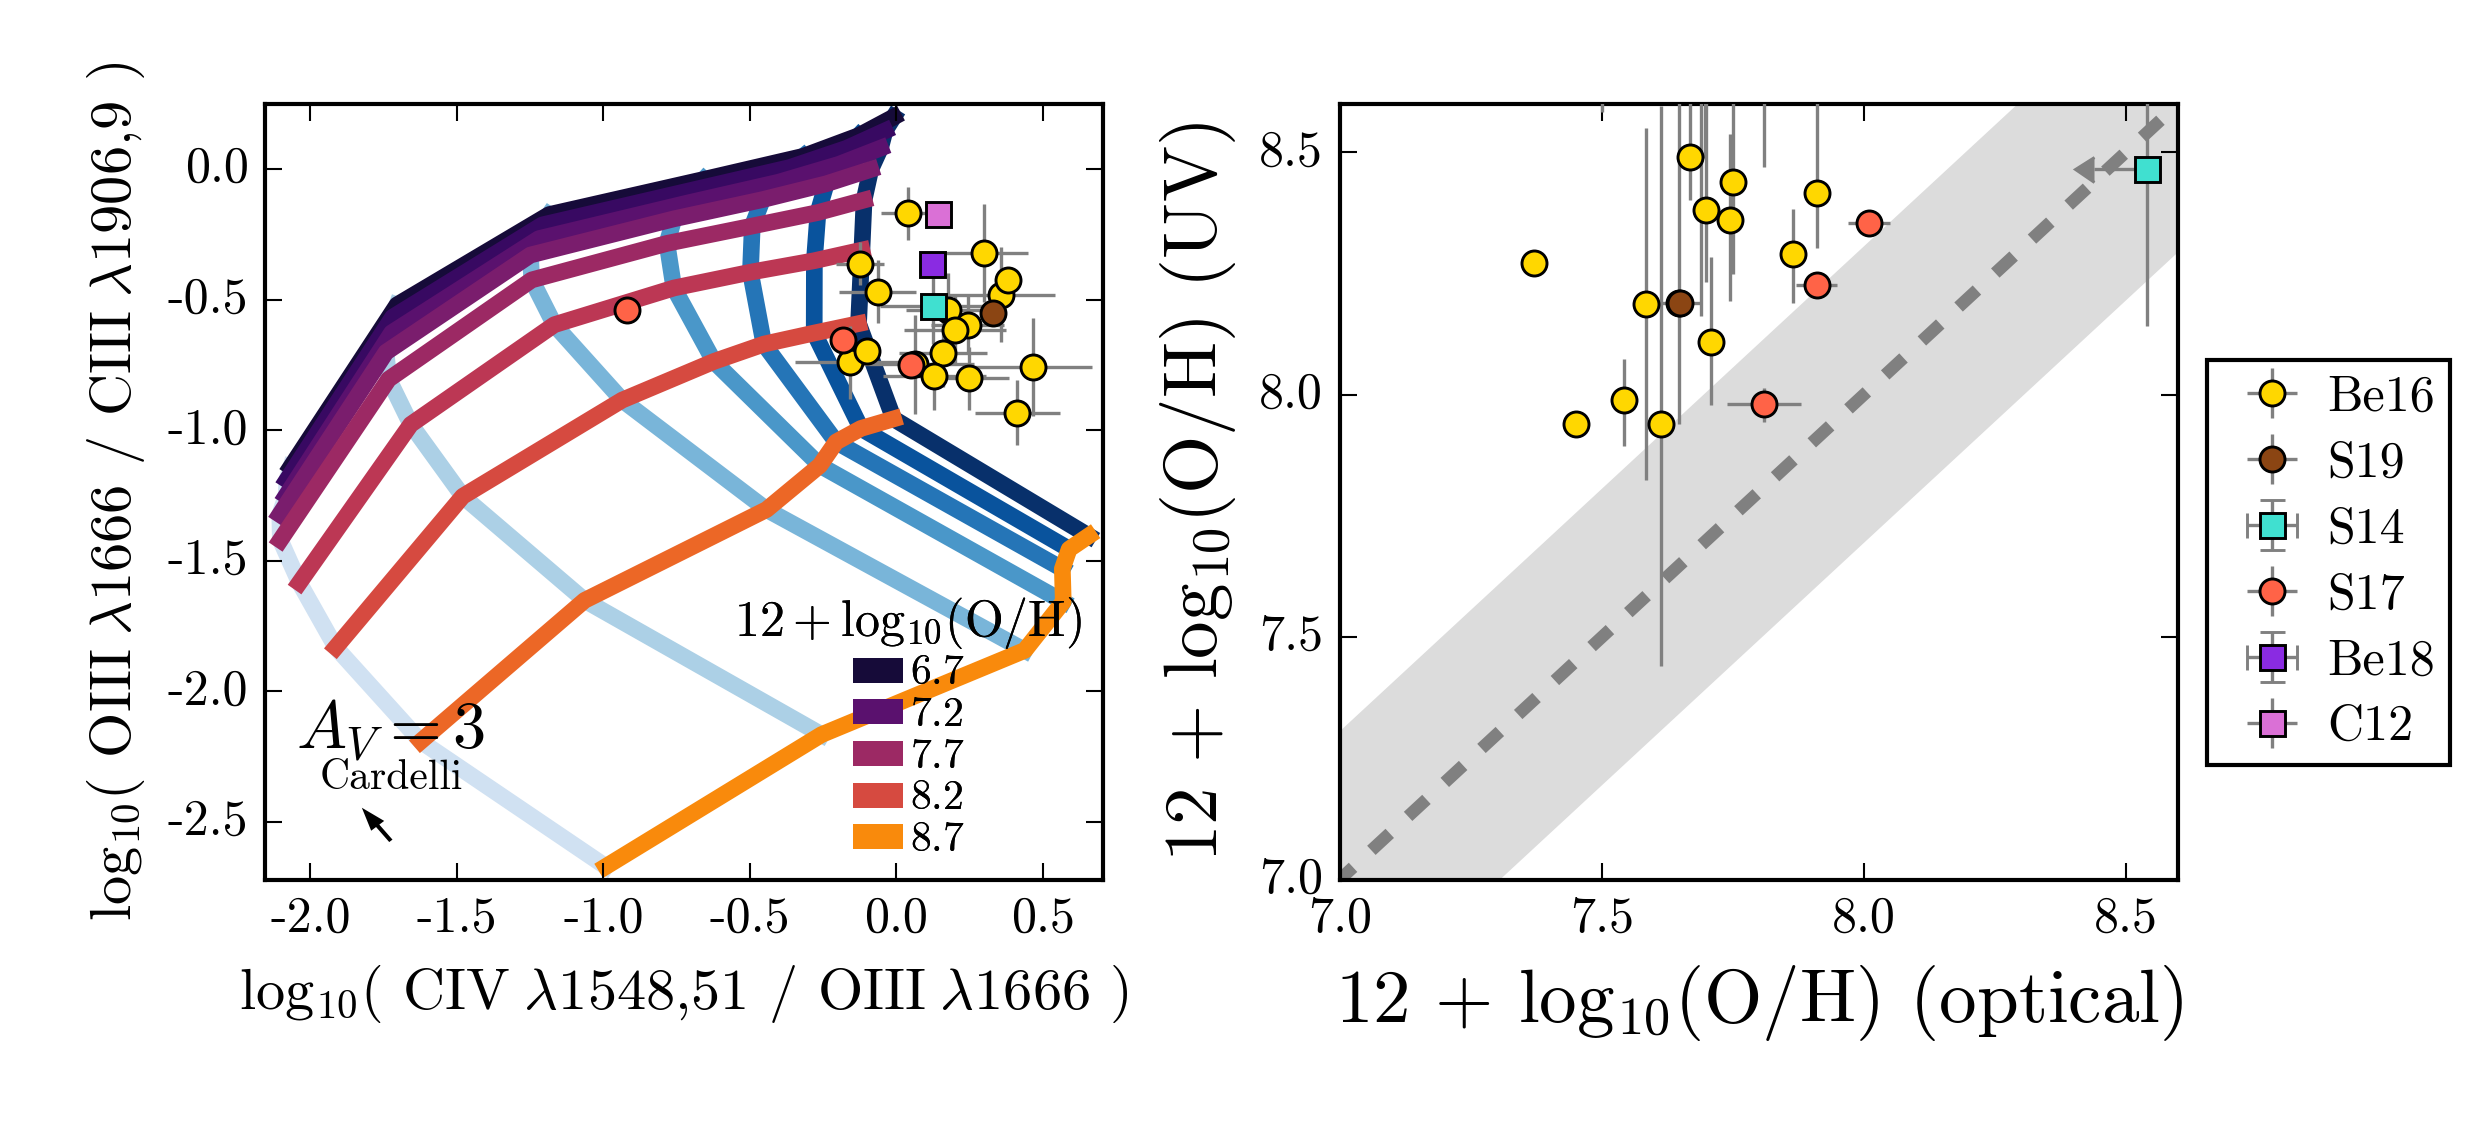
\includegraphics[width=\linewidth]{figs/f5.png}
    \caption{UV diagnostic diagrams using pairs of emission lines excluding carbon species and \heii$\lambda$1640.  The blue lines connect models of constant ionization parameter, from \logUeq{-1} (dark blue) to \logUeq{-4} (light blue). Models of constant metallicity are shown from \logZeq{-2} (purple) to \logZeq{0} (orange). The colored diamonds show the high-redshift galaxies from \citet{Rigby+2018b}. There are few galaxies where all four emission lines used in a given diagnostic diagram are observed in multiple objects. For galaxies that appear in multiple diagrams, the position in ionization parameter - metallicity space is roughly consistent between diagnostics.}
    \label{fig:UVSiO}
  \end{center}
\end{figure*}
%-------------------------------------------------------

In Fig.~\ref{fig:UVZ} we compare the optical metallicity of RCS0327 and S1527 to various UV metallicities, as derived using different diagnostics. The optical metallicity is shown on the $x$-axis, while the UV metallicity is shown on the $y$-axis. The marker color indicates the specific UV diagnostic used, labeled on the color bar. While RCS0327 has a single optical metallicity measurement, the rest-UV spectroscopy targets multiple spatial locations corresponding to several distinct star-forming knots. We separate the knots (E,G, U) on the $x$-axis of Fig.~\ref{fig:UVZ} for visual clarity, with an offset of $\pm 0.1$\,dex from the globally averaged optical metallicity, shown at the location of knot-G. The knots are also separated because, in principle, the gas properties could vary significantly between knots. We leave this analysis to a future publication, Byler et al., \emph{in prep}.

We can see from Fig.~\ref{fig:UVZ} that the UV-derived metallicities are consistent with the optical metallicities, within error. The consistency between the UV and optical metallicities in Fig~\ref{fig:UVZ} may indicate that UV diagnostics using silicon and oxygen lines are more robust than those using carbon or helium emission lines.

In general, the various UV metallicities for each object agree with one another, with a scatter of 0.2-0.3\,dex. However, as discussed in \S\ref{sec:ZZ:UVOpt}, some of the diagnostics provide less reliable metallicity estimates. We found that the Si2Si2-Si2Si3 diagnostic (light blue diamonds in Fig.~\ref{fig:UVZ}) produced metallicities that were systematically higher than other diagnostics. The Si2Si2-Si2Si3 lines were all observable in RCS0327-U and S1527, shown in Fig.~\ref{fig:UVZ}. For RCS0327 the Si2Si2-Si2Si3 metallicity shows the largest offset from the optical metallicity, more than 0.5\,dex. For S1527, the Si2Si2-Si2Si3 diagnostic predicts a metallicity at the upper limit set by the optical \nii/\ha ratio. In both cases, it is reasonable to claim that the Si2Si2-Si2Si3 metallicity is biased to systematically high metallicities.

The best of the diagnostics identified in \S\ref{sec:ZZ:UVOpt} included Si2Si2-O3Si3 (bright green), Si2O3-Si3O2 (brown), Si2Si2-N3Si3 (pale orange), and Si2Si2-O2O3 (pale red). In Fig.~\ref{fig:UVZ}, these diagnostics show very little scatter in individual objects, (e.g., the pale red and bright green diamonds for knot-G), by design. We also note that these diagnostics provide the closest match to the measured optical metallicity in several objects, which is encouraging.

%-------------------------------------------------------
% Figure 7:
%-------------------------------------------------------
\begin{figure*}
  \begin{center}
    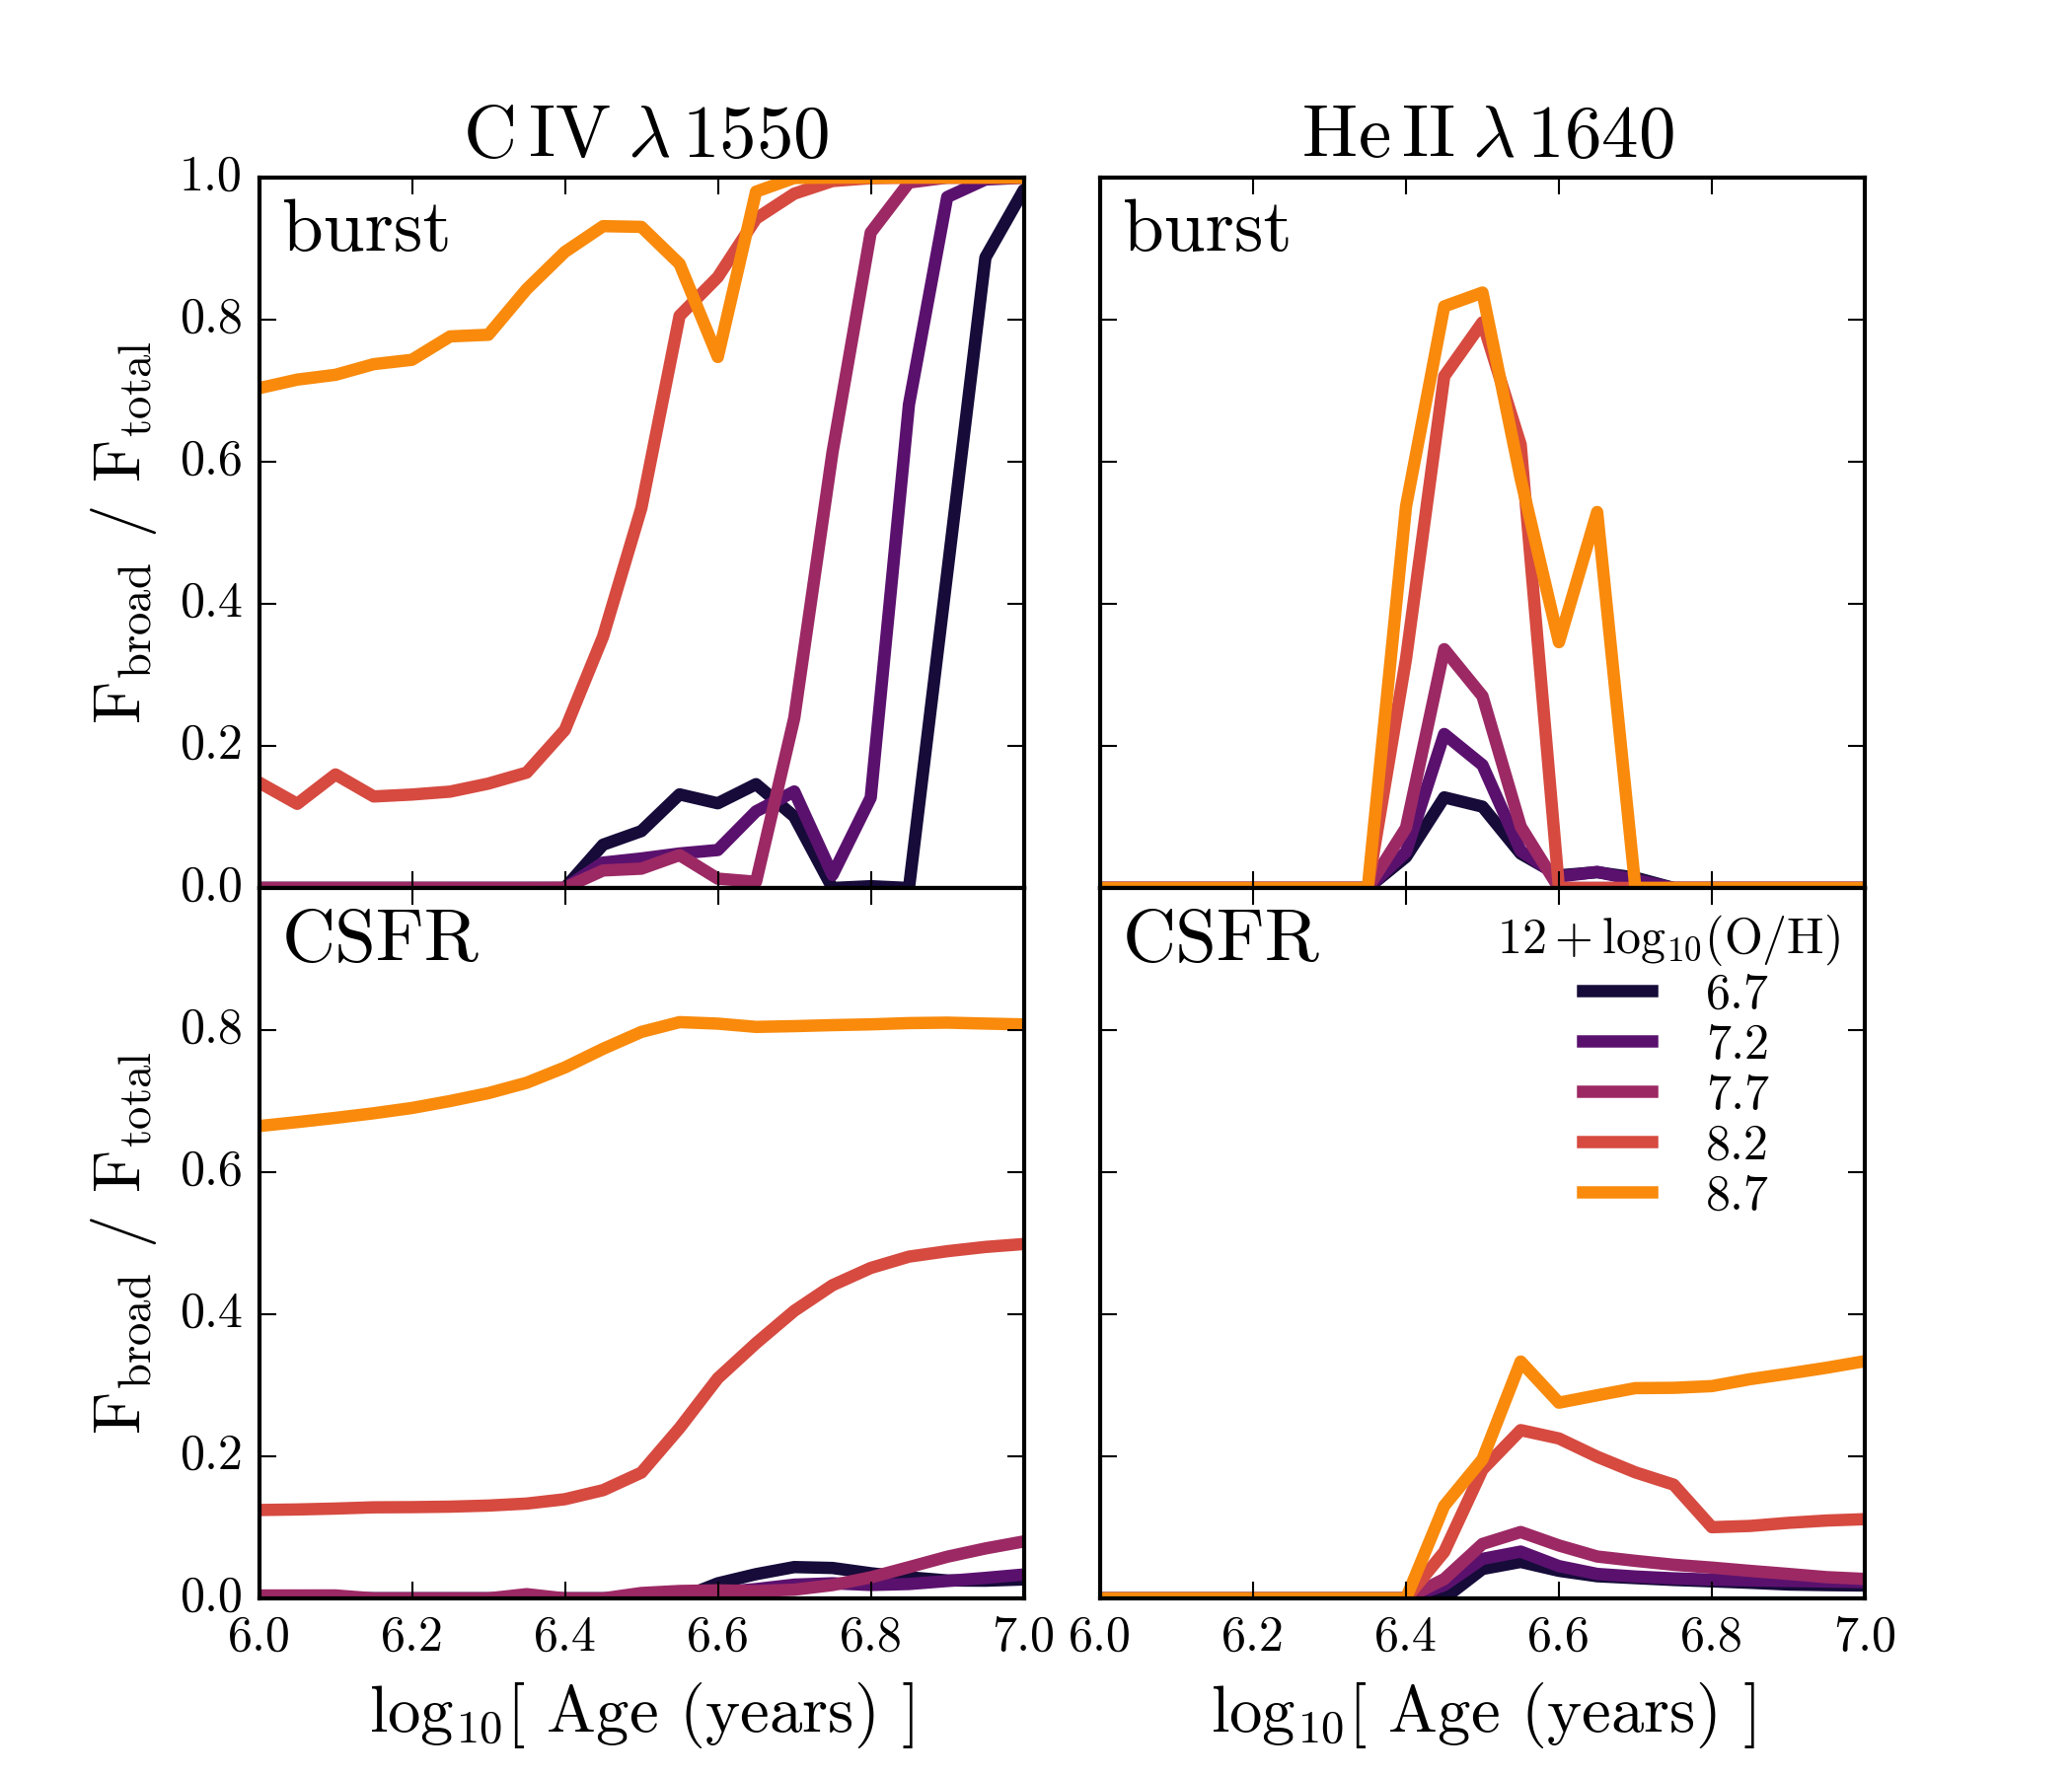
\includegraphics[width=\linewidth]{figs/f7.png}
    \caption{UV metallicities ($y$-axis) derived from various diagnostic diagrams compared to the optical metallicity ($x$-axis). Marker color indicates the different emission line ratios used, and the red dashed line shows a one-to-one relation. RCS0327 has a single optical metallicity measurement spatially averaged over the face of the galaxy, but rest-UV spectra that cover several different spatial locations (e.g., U,G,E,B), which have been shifted on the $x$-axis for visual clarity. The optical metallicity for S1527 only provides an upper limit.}
    \label{fig:UVZ}
  \end{center}
\end{figure*}
%-------------------------------------------------------

\subsection{UV-UV abundance comparisons}\label{sec:ZZ:UV}

We quantify the robustness of the UV metallicities by looking for consistent predictions between different UV diagnostics. For this consistency check, we use the 12 UV diagnostics identified in Table~\XXX.

Fig.~\ref{fig:UVUV} shows the gas phase oxygen abundance predicted by each of the 12 diagnostics, compared with the oxygen abundance derived using each of the 11 other diagnostics. The rows and columns are labeled with the diagnostic plotted on the $x$- and $y$-axis, respectively. The red dashed line represents unity, and the \mage galaxies are shown with colored diamonds, as indicated in the figure legend.

It is evident from Fig.~\ref{fig:UVUV} that some diagnostics are more consistent than others. For example, the \SiuII$\lambda$1307/\SiuII$\lambda$1531 \vs \SiuII$\lambda$1307/\SiuIII$\lambda$1883 diagnostic (Si2Si2-Si2Si3; first column, $y$-axis) predicts metallicities that are systematically higher than those predicted by other diagnostics by 0.2-0.4\,dex. Encouragingly, though, there are a number of diagnostics that predict metallicities that are well-matched with predictions from other diagnostics. The \SiuII$\lambda$1307/\SiuII$\lambda$1531 \vs \oiii$\lambda$1666/\SiuIII$\lambda$1883 diagnostic (Si2Si2-O3Si3; third row, $x$-axis, and fourth column, $y$-axis) is quite promising, because these emission lines are observed in a number of galaxies and the predicted metallicities agree with several other diagnostics.

In general, the diagnostics using a single species (e.g., all silicon lines) have the least consistent metallicity predictions. Diagnostics that include a mix of ionization states (e.g. \oiii and \oii) seem to produce more consistent metallicity predictions. From Fig.~\ref{fig:UVUV}, other promising diagnostics include:
\begin{itemize}
    \item \SiuII$\lambda$1307/\oiii$\lambda$1666 \vs \SiuIII$\lambda$1883/\oii$\lambda$2471 (Si2O3-Si3O2; 11th row, $x$-axis and 12th column, $y$-axis)
    \item \SiuII$\lambda$1307/\SiuII$\lambda$1531 \vs \niii1750/\SiuIII1883 (Si2Si2-N3Si3; 6th row $x$-axis, 7th column $y$-axis)
    \item \SiuII$\lambda$1307/\SiuII$\lambda$1531 \vs \oii$\lambda$2471/\oiii$\lambda$1666 (Si2Si2-O2O3; 4th row $x$-axis, 5th column $y$-axis)
\end{itemize}

Only one galaxy has observed \mgii$\lambda$2796 emission. The diagnostic that includes \mgii$\lambda$2796 also produces systematically low metallicity estimates. However, the \mgii$\lambda$2796 emission may not have a nebular origin; \citet{Rigby+2018a} suggests the \mgii$\lambda$2796 emission is the result of continuum upscattering.

%-------------------------------------------------------
% Figure 6:
%-------------------------------------------------------
\begin{figure*}
  \begin{center}
    \includegraphics[width=\linewidth]{figs/f6.png}
    \caption{Consistency between UV-derived metallicities. We show the gas phase oxygen abundance ($12+$\logOH) measured with twelve different UV-diagnostics, as labeled on the outer edges of the figure. The diagnostic labeled on each row is plotted on the $x$-axis, while the diagnostic labeled on the columns is plotted on the $y-$axis. \mage galaxies are shown with colored diamonds and the red dashed line shows a one-to-one relationship. The \SiuII$\lambda$1307/\SiuII$\lambda$1531 \vs \oiii$\lambda$1666/\SiuIII$\lambda$1883 diagnostic (the third row, $x$-axis and the fourth column, $y$-axis) predicts metallicities that are consistent with most other diagnostics. In contrast, the \SiuII$\lambda$1307/\SiuII$\lambda$1531 \vs \SiuII$\lambda$1307/\SiuIII$\lambda$1883 diagnostic (first column, $y$-axis) predicts metallicities that are systematically higher than other diagnostics.}
    \label{fig:UVUV}
  \end{center}
\end{figure*}
%-------------------------------------------------------

 from discussion:
 
In the right panel of Fig.~\ref{fig:CO}, we show the same UV-optical metallicity comparison, now color-coded by the \oiii electron temperature. The same two objects with overestimated metallicities and different C/O ratios have very similar temperatures, and the largest temperatures found in the \citet{Berg+2016} sample.

Hotter nebulae produce stronger \ciii emission, which would decrease both the Si3C3 and O3C3 ratios at fixed oxygen abundance, pushing objects toward higher metallicity models. We would expect the \ciii lines to be much more sensitive to the presence of shock heating than the optical \oiii lines, potentially explaining the overestimated metallicities from the Si3C3-O3C3 diagnostic. We plan to more thoroughly explore this explanation in future work.
%Moreover, \citet{Dopita+1997} noted that these collisionally-excited lines should be a useful probe of shock-heated gas. Shock models predict stronger \ciii emission fluxes than either AGN or SF models. It is possible that the discrepant metallicities derived with the Si3C3-O3C3 diagnostic reflect the temperature sensitivity of the \ciii lines.


\section{UV-derived metallicities}\label{sec:UVZ}

In this section, we derive metallicities for the \mage galaxies using the most promising set of diagnostics from \S\ref{sec:ZZ:UV}. The \mage galaxies with both UV and optical metallicities can be used to connect studies where only optical or only UV metallicities are available. We first derive metallicities using all 12 diagnostics used in this work. We then propose a new weighting scheme based on the post promising subset of diagnostics identified in \S\ref{sec:ZZ:UVOpt}, and then calculate UV metallicities for the \mage sample.

Fig.~\ref{fig:UVmage} shows the gas phase oxygen abundance derived using all 12 UV diagnostics for each of the \mage galaxies. Each point is color-coded by the diagnostic used to derive the abundance, using the same scheme as Fig.~\ref{fig:UVZ}, as indicated in the color bar. The diagnostics predict oxygen abundances between $7.75< 12+$\logOH$<8.75$. The spread in predicted metallicities for a given object varies between 0.25 dex and 0.75 dex.

As expected, in Fig.~\ref{fig:UVmage}, the Si2Si2-Si2Si3 diagnostic (pale blue diamonds) predicts the largest oxygen abundances in every object, offset from other predictions by at least $\sim0.25$ dex, and in an extreme case, by as much as 1\,dex. The metallicities predicted with this diagnostic exceed solar metallicity in most cases, which corresponds to gas enrichment that may be difficult to attain at the metallicities in this sample.

The best of the diagnostics identified in \S\ref{sec:ZZ:UV} included Si2Si2-O3Si3 (bright green diamonds), Si2O3-Si3O2 (brown), Si2Si2-N3Si3 (pale orange), and Si2Si2-O2O3 (pale red). When simultaneously measured in a single object, the spread in predicted metallicity is small, as expected.

From our analysis in \S\ref{sec:ZZ:UVOpt}, Si2Si2-O3Si3, Si2O3-Si3O2, Si2Si2-N3Si3, and Si2Si2-O2O3 produce the most accurate and precise metallicity estimates. To calculate a final UV metallicity for the galaxies in the \mage sample, we thus propose a weighted average of the metallicities derived with these four diagnostics, following the form \XXX; these metallicities are given in Table.\XXX.

Fig.~\ref{fig:UVmage} shows the "final" UV metallicity calculated for each of the \mage galaxies, now plotted as a function of redshift. For comparison, we also compare the metallicities and redshifts from blah (\XXX actually make this plot; not sure if this is the best way to summarize results).

%-------------------------------------------------------
% Figure 8:
%-------------------------------------------------------
\begin{figure*}
  \begin{center}
    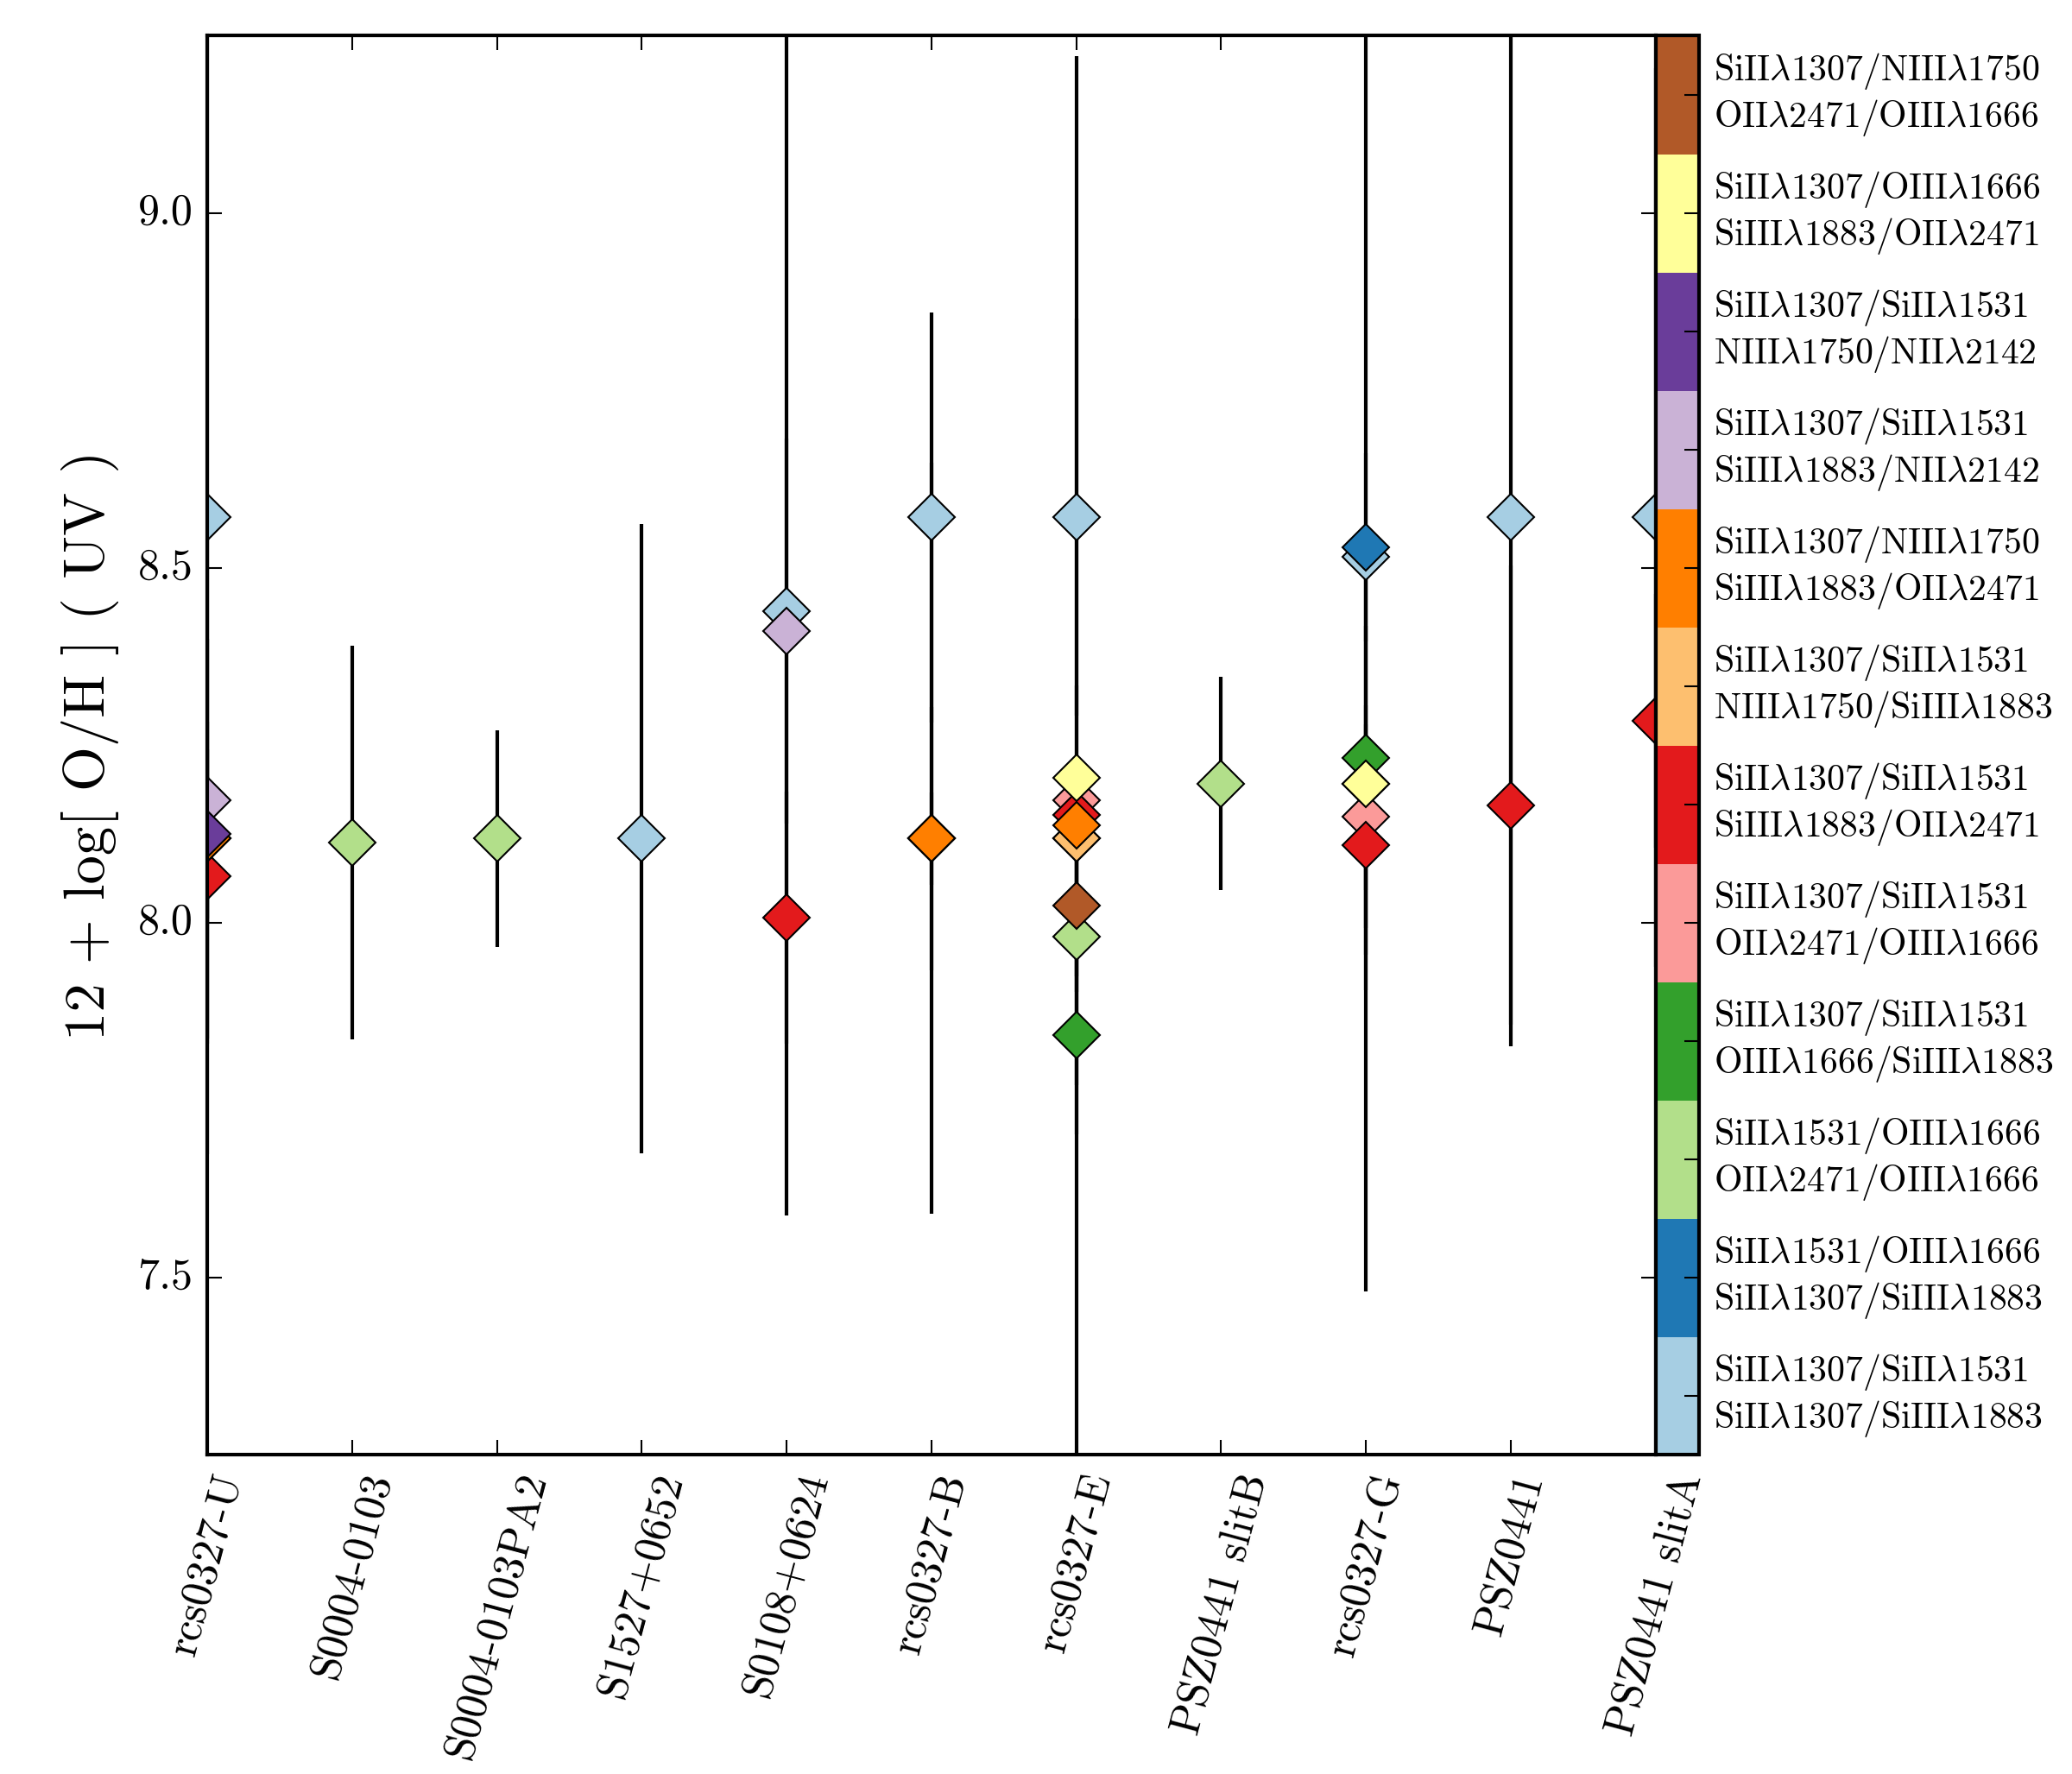
\includegraphics[width=\linewidth]{figs/f8.png}
    \caption{UV-derived metallicities ($y$-axis) for the \mage galaxies, each object is offset on the $x$-axis arbitrarily. Each marker is is color-coded by the diagnostic diagram used to derive the metallicity, as shown in the colorbar. }
    \label{fig:UVmage}
  \end{center}
\end{figure*}
%-------------------------------------------------------


conclusions:

    %\item We have confirmed that UV and optical direct-temperature oxygen abundances agree within 0.1-0.2dex. The UV direct-\Te abundances are systematically lower than the optical-\Te abundances by 0.1 dex, which increases to a 0.2\,dex offset at solar and super-solar metallicities.
        %\item UV metallicity diagnostics that include the \ciii$\lambda$1906,1909 emission lines do not reliably correlate with optical metallicities. We suggest that this is likely driven the presence of shock heated gas in addition to variations in C/O at fixed oxygen abundance.
    %\item UV diagnostics that consist of ratios of silicon, oxygen, and nitrogen emission lines spanning multiple ionization states provide the most reliable metallicity estimates, like \SiuII$\lambda$1307/\SiuII$\lambda$1531 \vs \oiii$\lambda$1666/\SiuIII$\lambda$1883. Other promising diagnostics include \SiuII$\lambda$1307/\oiii$\lambda$1666 \vs \SiuIII$\lambda$1883/\oii$\lambda$2471, \SiuII$\lambda$1307/\SiuII$\lambda$1531 \vs \niii$\lambda$1750/\SiuIII$\lambda$1883, and \SiuII$\lambda$1307/\SiuII$\lambda$1531 \vs \oii$\lambda$2471/\oiii$\lambda$1666.
    %\item Using the \mage galaxy sample, we demonstrate that metallicities derived using the above diagnostics are consistent with optical metallicities derived using empirically calculated strong line indices. Additionally, the metallicities derived using these diagnostics are consistent with metallicities derived using other UV diagnostics.
    %\item We have calculated UV metallicities for the \mage galaxies using a weighted average of the five diagnostics presented above.
\section{Caveats}\label{sec:caveats}
%Silicon emission lines proved to be fairly unreliable metallicity tracers. Metallicity diagnostics that involve silicon lines tend to overestimate the metallicity, by as much as 1\,dex in extreme cases. There are a few possible explanations for the mismatch between observed and model-predicted silicon line ratios, including: (1) incorrect silicon abundances (both the total gas phase abundance and the fraction depleted onto dust grains), (2) incorrect atomic data, (3) the sensitivity of the silicon ionization energy to age and metallicity variations in ionizing flux, and (4) possible contamination from supernovae (SNe) emission. We briefly discuss each of these explanations in turn.

\paragraph{Depletion Factors} 
\paragraph{Atomic data}
\paragraph{Diffuse Ionized gas}
\paragraph{Continuum fits}
\paragraph{Stellar and nebular abundances}

%Optical metallicity estimates for these seven galaxies are compiled in Table 2 of \citet{Rigby+2018b}, which are calculated from strong line methods, either the $R_{23}$ or O3N2 indices \citep{Pettini+2004} and corrected to the PP04-N2 system following \citet{Kewley+2008}. We describe the method used to calculate uniform optical metallicities in \S\ref{sec:Z:corr:strong}.


%do not, where we would expect the influence of broad emission to be the most important. Visual inspection of the \mage galaxy \heii spectral features does show relatively broad line profiles, \todo{FIX: but the contamination must not provide any additional metallicity leverage}.

%\subsubsection{Wind-contaminated \civ$\lambda$1550}
%
%Out of all the diagnostics presented in this work, the UV diagnostics that include the \civ$\lambda$1548,1550 lines preform the worst, predicting metallicities that are systematically 0.2-0.6\,dex larger than optical metallicities. Much of the failure can be attributed to the mismatch between predicted and observed C4O3 ratios, where observed C4O3 ratios are larger.
%
%It is not unreasonable to think that stellar wind emission could be inflating measured \civ fluxes. In the \mage galaxies, there is little evidence for nebular emission and only stellar \civ emission is detectable. For the \citet{Berg+2016} galaxies, the \civ$\lambda$1548,1550 lines are broader than the other nebular emission lines, consistent with the presence of stellar wind emission. The \citet{Senchyna+2017} observations are the only observations that we can be confident are ``nebular only,'' because the spectral resolution of the observations was high enough to decipher broad and narrow \civ components. 
%